\documentclass[runningheads]{llncs}
\usepackage{graphicx}
\usepackage{url}
\usepackage{mathtools,textcomp}
\usepackage[noend]{algpseudocode}
\usepackage{multirow}
\usepackage{caption}
\captionsetup[table]{skip=10pt}
% Used for displaying a sample figure. If possible, figure files should
% be included in EPS format.
%
% If you use the hyperref package, please uncomment the following line
% to display URLs in blue roman font according to Springer's eBook style:
% \renewcommand\UrlFont{\color{blue}\rmfamily}

\begin{document}
\title{MongoDB for Credit Card Fraud Detection}

\author{Davide Cazzetta\orcidID{976585} \and Riccardo Giussani\orcidID{973238}}

\authorrunning{Davide \& Riccardo}
% First names are abbreviated in the running head.
% If there are more than two authors, 'et al.' is used.
%
\institute{Università degli Studi di Milano Statale, Milan MI 20133, Italy \\
\url{https://www.unimi.it/it/corsi/corsi-di-laurea/informatica-magistrale}}
%
\maketitle              % typeset the header of the contribution
%
\begin{abstract}
The abstract should briefly summarize the contents of the paper in
150--250 words.

\keywords{First keyword  \and Second keyword \and Another keyword.}
\end{abstract}

\section{Introduction}

\subsection{Motivation}

Payment card fraud is a major challenge for business owners, payment card issuers, and transactional services companies, causing every year substantial and growing financial losses. Many Machine Learning approaches have been proposed in the literature that tries to automate the process of identifying fraudulent patterns from large volumes of data. The focus of this project aims at this last part: we exploit some algorithms that generate data about transactions to store these data into a NoSQL Database, specifically MongoDB\footnote{https://www.mongodb.com/}. In detail we want to see how does this system behave in the presence of large amount of data, evaluating the execution times for some operations.

\subsection{Conceptual Model}
In this scenario there are two stand-alone entities, that are \textbf{Customer} and \textbf{Terminal}, linked by the relationship \textbf{Transaction} when an event of this kind occurs. The two are also related through \textbf{available\_terminal}, relationship that subsists whether in our model the Customer can reach a Terminal to execute a Transaction.
\begin{figure}[!htb] 
        \centering 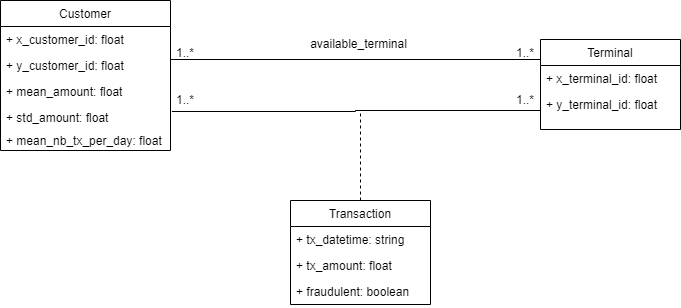
\includegraphics[width=0.9\columnwidth]{images/FraudDetectionUML.png}
        \caption{\label{fig1}UML of the generated data}
\end{figure}
\\
In a relational database, \textbf{Transaction} would be the join table between \textbf{Customer} and  \textbf{Terminal}
\\
Constraints e supposizioni:
\begin{enumerate}
    \item customers and terminals are unique
    \item a transaction is uniquely identified by the terminal on which it happened and the timestamp
    \item a transaction by a customer on a terminal can happen if and only if the relationship \textbf{available terminal} occurs among the two
    \item \textbf{available terminal} occurs among a customer and a terminal if and only if the terminal's coordinates lie within a certain range from the customer's
    \item geographical coordinates are real numbers between 0 and 100
\end{enumerate}

\section{Logical Model}
\subsection{Baseline Model}
Transactions are the core entity of the scenario (and consequently of the workload) and therefore all transactions are stored in a dedicated collection.
\\
After ingesting data into the database we compute the cardinalities of the relationships (minimum, average and maximum) to grasp a general idea on how much data we have to deal with and how it scales.
\\
qui una bella tabella!
\\
\begin{figure}[!htb] 
        \centering 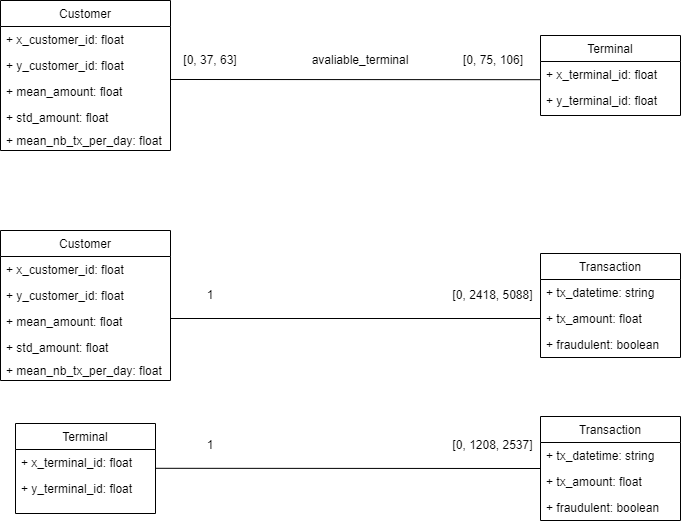
\includegraphics[width=0.9\columnwidth]{images/MongoCardinality.png}
        \caption{\label{fig2}Cardinalità delle relazioni; va bene così perchè card C-T è diversa da quella T-T}
\end{figure}
The \textbf{available\_terminal} relationship have manageable cardinalities on both sides. The data generating script already provides the list of terminals for each customer and therefore this navigability is maintained by reference on the \textbf{Customer} side.
\\
Queries tell us how we should theoretically navigate relationships:
\begin{enumerate}
    \item[a)] requires navigability from \textbf{Customer} to \textbf{Transaction}, to compute the sum
    \item[b)] requires to navigate from \textbf{Terminal} to \textbf{Transaction}, in order to compute the average
    \item[c)] requires both the navigability from \textbf{Customer} to \textbf{Terminal} and vice versa
    \item[d)] only requires transactions data
    \item[e)] only requires transactions data
\end{enumerate}
We notice however that maintaining a relationship with endpoint in \textbf{Transaction} is absolutely impractical as it represents the "many-side" of the relationships with a cardinality of potentially "zillions". Also, data of customers and terminals are not needed in the queries, therefore no embedding is required. For our baseline model, the reference from \textbf{Transaction} to \textbf{Customer} and \textbf{Terminal} through \emph{CUSTOMER\_ID} and \emph{TERMINAL\_ID} is sufficient.
\begin{figure}[!htb] 
        \centering 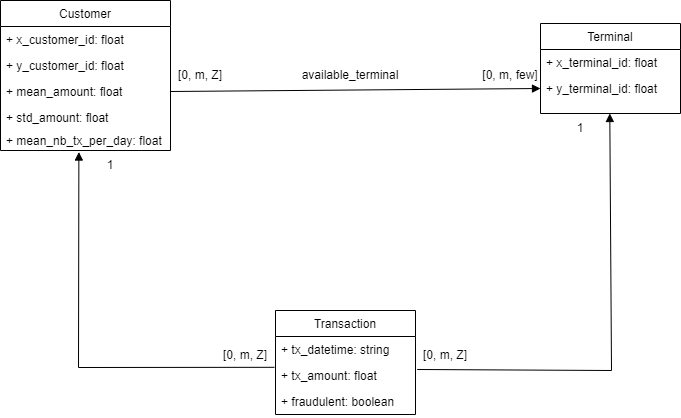
\includegraphics[width=0.9\columnwidth]{images/MongoBaselineNavigability.png}
        \caption{\label{fig3}Questa è la navigabilità baseline, solo guardando le query. Poi bisogna vedere le cardinalità}
\end{figure}
Later, some design patterns to speed up computation will be investigated.
% Please add the following required packages to your document preamble:
% \usepackage{multirow}
\begin{table}[]
\begin{tabular}{|c|cc|}
\hline
\multirow{2}{*}{} & \multicolumn{2}{c|}{available\_terminal}           \\ \cline{2-3} 
                  & \multicolumn{1}{c|}{customer side} & terminal side \\ \hline
average           & \multicolumn{1}{c|}{75}            & 37            \\ \hline
max               & \multicolumn{1}{c|}{106}           & 63            \\ \hline
\end{tabular}
\end{table}
% Please add the following required packages to your document preamble:
% \usepackage{multirow}
\begin{table}[]
\begin{tabular}{|cc|c|c|}
\hline
\multicolumn{2}{|c|}{\multirow{2}{*}{}}                    & \multirow{2}{*}{customer-transaction} & \multirow{2}{*}{terminal-transaction} \\
\multicolumn{2}{|c|}{}                                     &                                       &                                       \\ \hline
\multicolumn{1}{|c|}{\multirow{2}{*}{Dataset 1}} & average & 77                                    & 38                                    \\ \cline{2-4} 
\multicolumn{1}{|c|}{}                           & max     & 179                                   & 95                                    \\ \hline
\multicolumn{1}{|c|}{\multirow{2}{*}{Dataset 2}} & average & 231                                   & 115                                   \\ \cline{2-4} 
\multicolumn{1}{|c|}{}                           & max     & 520                                   & 263                                   \\ \hline
\multicolumn{1}{|c|}{\multirow{2}{*}{Dataset 3}} & average & 538                                   & 268                                   \\ \cline{2-4} 
\multicolumn{1}{|c|}{}                           & max     & 1200                                  & 586                                   \\ \hline
\end{tabular}
\end{table}
\section{Ingestion Layer}

The code is available at the following url \url{https://github.com/Davydhh/DBMS-Project.git}.

\hfill

\noindent
The ingestion layer is responsible for generating the datasets which will then be stored in MongoDB.

\subsection{Generate datasets}

The system can generate three datasets, one about customers, one related to terminals and the third regarding transactions. To generate these datasets we have exploited the scripts presented in this article: \url{fraud-detection-handbook.github.io/fraud-detection-handbook/Chapter_3_GettingStarted/SimulatedDataset.html}. In particular we have created a class \emph{DatasetsGenerator} where the user can pass the parameters \emph{start\_date} which represents the day on which transactions begin and \emph{nb\_days}, that is days of transactions. The decision to make only these two parameters arbitrary is due to the fact that the biggest dataset is about transactions, on the other hand the customers and terminals dataset are are much smaller in comparison, as a result, the customer and terminal parameters are constant at 5000 and 10000 respectively.
\\
The objective of the work is to generate three datasets each composed of the three datasets described above, to do this we started with a base of 5000 customers, 10000 terminals and 40 days of transactions (starting from the date 2022-01-01) and then, at each iteration, the start date is increased by one year and the days of transactions are doubled. The following datasets were generated in this way:

\begin{enumerate}
    \item \begin{itemize}
        \item customers: 3 MB
        \item terminals: 1 MB
        \item transactions (2018): 330 MB
    \end{itemize}
    \item \begin{itemize}
        \item customers: 3 MB
        \item terminals: 1 MB
        \item transactions (2019): 670 MB
    \end{itemize}
    \item \begin{itemize}
        \item customers: 3 MB
        \item terminals: 1 MB
        \item transactions (2020): 1.3 GB
    \end{itemize}
\end{enumerate}

\subsection{Store data in MongoDB}

The second part of the ingestion layer consists of saving the data in MongoDB. The datasets are generated in json format to facilitate saving in the database; in fact the data are stored with the \emph{updateMany\footnote{https://docs.mongodb.com/manual/reference/method/db.collection.updateMany/}} method. In particular, transaction data are saved at each iteration, whereas customer and terminal datasets are only saved at the first iteration as they are the same for all three generated datasets.

\section{Queries}

This section explains in detail how the queries were implemented to obtain the required results.

\subsection{Query A}

\emph{For each customer identifies the amount that he/she has spent for every day of the current month.}

\hfill

Since with have noticed that the \emph{TX\_DATETIME} field is saved in Mongo in milliseconds as type Int the first step is convert this field into Datetime format in order extract days and months from the date. The  convertion into Datetime type was made with the \emph{\$toDate\footnote{https://docs.mongodb.com/manual/reference/operator/aggregation/toDate/}} method inside a \emph{\$project\footnote{https://docs.mongodb.com/manual/reference/operator/aggregation/project/}} stage and then we have extracted the day and the month with the \emph{\$dayOfMonth\footnote{https://docs.mongodb.com/manual/reference/operator/aggregation/dayOfMonth/}} and \emph{\$month\footnote{https://docs.mongodb.com/manual/reference/operator/aggregation/month/}} methods respectively.\\
The second step is filter data about the current month through a \emph{\$match} stage; to obtain the current month the \emph{datetime\footnote{https://docs.python.org/3/library/datetime.html}} Python library has been used.\\
The last step consists in grouping the data by user and by day by summing the \emph{TX\_AMOUNT} field with the \emph{\$group\footnote{https://docs.mongodb.com/manual/reference/operator/aggregation/group/}} and \emph{\$sum\footnote{https://docs.mongodb.com/manual/reference/operator/aggregation/sum/}} methods.

The resulting query consists of a pipeline aggregation on the transactions collection.

\subsection{Query B}

\emph{For each terminal identify the possible fraudulent transactions. The fraudulent transactions
are those whose import is higher than 50\% of the average import of the transactions
executed on the same terminal in the last month.}

\hfill

Since for each terminal we need to have all transactions, the \emph{\$lookup\footnote{https://docs.mongodb.com/manual/reference/operator/aggregation/lookup/}} method, starting from the terminals collection with the transactions collection, is very useful for this purpose. After that we have created another field (in a \emph{\$project} stage) named \emph{transactions\_avg} which we could process to calculate the average import of the transactions. Specifically, as a first step we eliminated the terminals that had no transactions in the last 30 days through a \emph{\$match} method where the last 30 days were obtained again through the \emph{datetime} library, than the method \emph{\$filter\footnote{https://docs.mongodb.com/manual/reference/operator/aggregation/filter/}} inside a \emph{\$project} stage was used to get only the transactions executed in the last month. At this point it was possible to obtain the value relative to 50\% of the average import of the transactions with the \emph{\$avg} and \emph{\$divide\footnote{https://docs.mongodb.com/manual/reference/operator/aggregation/divide/}} methods.\\
Finally, the last operations to be carried out served to obtain the fraudulent transactions because for each terminal we now have the reference to the threshold value; a \emph{\$match} and \emph{\$project} stages are exploited to get only transactions whose import is higher than the \emph{transactions\_avg} field.\\

The resulting query consists of a pipeline aggregation on the terminals collection.


\subsection{Query C}
\emph{Given a user u, determine the “co-customer-relationships CC of degree k”. A user u’ is a co-customer of u if you can determine a chain “$u_1-t_1-u_2-t_2- \ldots t_k-1-u_k$“ such that $u_1=u$, $u_k=u\textnormal{\textquotesingle}$, and for each 1<=I,j<=k, $u_i <> u_j$, and $t_1, \ldots t_k-1$ are the terminals on which a transaction has been executed. Therefore, $CC_k(u)={u'}$| a chain exists between u and u\textnormal{\textquotesingle} of degree k. Please, note that depending on the adopted model, the computation of $CC_k(u)$ could be quite complicated. Consider therefore at least the computation of $C_C3(u)$ (i.e. the co-costumer relationships of degree 3).}

\hfill

The determination of such a relationship would require, at an high-level perspective, the traversal of a graph where each customer is linked to each terminal that they had used at least once and vice versa. The only information explicitly reported in the database concerning the relationship among customers and terminals is the \textbf{available\_terminal} list embedded in each document of the \textbf{Customer} collection. This is however not sufficient, as we can't say whether the customer has used a terminal at least once and we'd also need to link each terminal to customers that have used it at least once.
\\
Getting for each terminal the customers that have used it requires a simple grouping over the \textbf{Transaction} collection by \emph{TERMINAL\_ID} that accumulates all the \textbf{CUSTOMER\_ID} in the set called \emph{cust\_used\_once} through the command \emph{\$addToSet\footnote{https://docs.mongodb.com/manual/reference/operator/aggregation/addToSet/}}
\\
As we are allowed to restrain ourself to compute only the relationship of degree 3, we opt for a simple set manipulation approach.\\
Given two terminals, each with its list of customers $cust\_used\_once_1$ and $cust\_used\_once_2$ (from now on simply $t_1$ and $t_2$), we identify three sets:
\begin{enumerate}
    \item $t_1 \cap t_2$: customers that have used both terminals
    \item $t_1 \setminus t_2$ customers that have used terminal 1 but not terminal 2
    \item $t_2 \setminus t_1$ customers that have used terminal 2 but not terminal 1
\end{enumerate}
Given the relationship definition of degree 3: 
\\
$u_1-t_1-u_2-t_2-u_3$
\\
Intuitively we see that customers in $t_1 \setminus t_2$ can only cover the role of $u_1$ and customers in $t_2 \setminus t_1$ the role of $u_3$. Those in $t_1 \cap t_2$ are the only ones that can be in the place of $u_2$. Note that the three sets are disjointed.
\\
We notice that it's sufficient that $t_1 \cap t_2$ is nonempty to determine that each customer in $t_1 \setminus t_2$ is a co-customer of degree 3 to each customer in $t_2 \setminus t_1$, as a "bridge" can be created. Also, if $|t_1 \cap t_2| > 1$ each customer in $t_1 \setminus t_2$ and each customer in $t_2 \setminus t_1$ is a co-customer of degree 3 to each customer in $t_1 \cap t_2$. At least, if $|t_1 \cap t_2| > 2$ each customer in $t_1 \cap t_2$ is a co-customer of degree 3 to each other customer in $t_1 \cap t_2$.
\\
We are only interested in co-customers for a user-given customer, therefore among all possible terminals we select as $t_1$ only those that have the specified customer inside.
\subsection{Query D}

\subsubsection{Point i}

\paragraph{1}

\emph{The period of the day \{morning, afternoon, evening, night\} in which the transaction has been executed.}

\hfill

The label corresponding to the period of the day strictly depends on the value of the field \emph{TX\_DATETIME}, precisely from the time of day, for this reason we have extracted the hour with the \emph{\$hour} method creating a new field using the \emph{\$addToField\footnote{https://docs.mongodb.com/manual/reference/operator/aggregation/addFields/}} method. After that we have generated a new field named \emph{period} which will contain the string representing the period of the day. To determine the value we use the Mongo command \emph{\$switch\footnote{https://docs.mongodb.com/manual/reference/operator/aggregation/switch/}}. The logic is:\\

\begin{algorithmic}
\If{$6 \geq $ hour $ \leq 12$} 
    \State $period \gets $morning
\Else
    \If{$12 < $ hour $ \leq 18$}
        \State $period \gets $ afternoon
\Else
    \If{$18 < $ hour $ \leq 22$}
        \State $period \gets $ evening
\Else
    \State $period \gets $ night
\EndIf
\EndIf
\EndIf
\end{algorithmic}

\paragraph{2}

\emph{The kind of products that have been bought through the transaction \{high-tech, food, clothing, consumable, other\}}

\hfill

Since we need to add a field whose content is to be generated automatically from a series of wordswe thought of applying a Javascript function to each row using the Mongo command \emph{forEach\footnote{https://docs.mongodb.com/manual/reference/method/cursor.forEach/}}. This method works but the library \emph{PyMongo} doesn't developed an API to use this Mongo function, so we have decided to do this in Python.\\
We have retrieved all transactions where the filed \emph{product\_kind} doesn't exist and then for each of them we have applied an \emph{updateOne\footnote{https://docs.mongodb.com/manual/reference/method/db.collection.updateOne/}} where the value of the field \emph{product\_kind} is chosen randomly from a list of possible choices.

\subsubsection{Point ii}

\emph{Customers that make more than three transactions related to the same types of products from the same terminal should be connected as “buying\_friends”. Therefore also this kind of relationship should be explicitly stored in the NOSQL database and can be queried.}

\hfill

We take into account the \textbf{Transaction} collection and specify an aggregation pipeline. As first step we \emph{\$group} by \emph{TERMINAL\_ID}, \emph{CUSTOMER\_ID} and \emph{product\_kind} and count the number of occurrences of each combination of values; then we \emph{\$match} only those triplets that have a count of occurrences strictly greater than 3. The last step requires a \emph{\$group} using as id \emph{TERMINAL\_ID} and \emph{product\_kind}. The accumulator function is an \emph{\$addToSet} that puts in a list (without duplication) all the \emph{CUSTOMER\_ID}.
\\
This pipeline returns, for each combination of \emph{TERMINAL\_ID} and \emph{product\_kind}, the customers that have made more than 3 transactions with those values. Notice that the \textbf{buying\_friend} relationship, in general, is not transitive and the cardinality can be too big to represent by reference all the ids of friends inside the customer document.
\\
\begin{figure}[!htb] 
        \centering 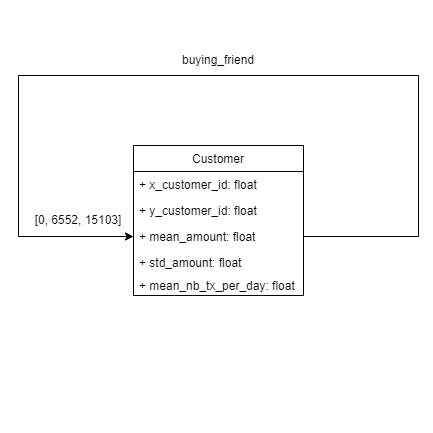
\includegraphics[width=0.5\columnwidth]{images/buyingFriends_all.png}
        \caption{\label{b_f_all}buying\_friend Relationship, not constrained by terminal and kind}
\end{figure}
When considering the same relationship constrained on terminal and product kind, we see that the cardinality is much smaller and it is transitive, which has the effect that a customer is buying friend to all customers that have bought the same product kind on the same terminal more than three times.\\
\begin{figure}[!htb] 
        \centering 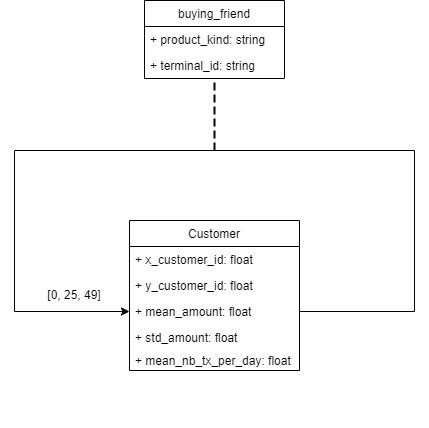
\includegraphics[width=0.5\columnwidth]{images/buyingFriends_base.png}
        \caption{\label{b_f_base}buying friend Relationship}
\end{figure}
We could therefore specify a new entity, \textbf{Buying\_Group}, toward which the \textbf{Customer} is linked to by a relationship \textbf{part\_of}. When a customer is a part of a group, they are friends with all other customers that are part of the same group.\\
The number of groups is of the same order of magnitude of the cardinality of \textbf{Terminal} and the references to customers are manageable.
\begin{figure}[!htb] 
        \centering 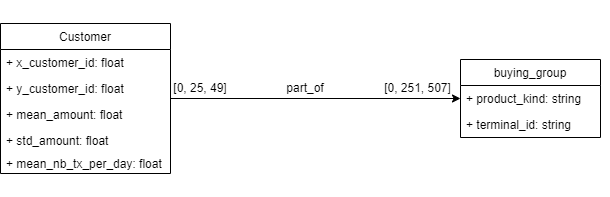
\includegraphics[width=0.8\columnwidth]{images/buyingFriends_group.png}
        \caption{\label{b_group}part\_of buying\_group relationship}
\end{figure}

\subsection{Query E}
\emph{For each period of the day identifies the number of transactions that occurred in that period, and the average number of fraudulent transactions.}

\hfill

\noindent
This query involves a simple \emph{\$group} stage by \emph{\$period} in aggregation where we use two accumulators: a \emph{\$sum}, to count the number of transactions, and \emph{\$avg\footnote{https://docs.mongodb.com/manual/reference/operator/aggregation/avg/}}, to compute the average number of fraudulent transactions.
\section{Performance}

To evaluate the performance we have calculated the execution times for all the previous operations.To do this, in the case of an aggregation, the database command \emph{explain\footnote{https://docs.mongodb.com/manual/reference/command/explain/\#mongodb-dbcommand-dbcmd.explain}} was used. In all other cases, e.g. for update operations, the time was obtained through the \emph{time\footnote{https://docs.python.org/3/library/time.html}} Python library, calculating the difference between the time the method finished and the time it started.\\
Performances (expressed in seconds) are as follows (note that every transactions dataset is added with the previous one, so at the first iteration we have transactions about 2018, at the second transactions about 2018 and 2019 and at the last iteration transactions about 2018, 2019 and 2020):


\begin{table}[!htb]
\centering
\begin{tabular}{l|c|c|c|ccc|c|l|}
\cline{2-9}
 &
  Query A &
  Query B &
  Query C &
  \multicolumn{3}{c|}{Query D} &
  Query E &
  Storing \\ \cline{2-9} 
\multirow{2}{*}{} &
  \multicolumn{1}{l|}{} &
  \multicolumn{1}{l|}{} &
   &
  \multicolumn{2}{c|}{Point i} &
  Point ii &
  \multicolumn{1}{l|}{} &
   \\ \cline{5-7}
 & \multicolumn{1}{l|}{} & \multicolumn{1}{l|}{} &  & \multicolumn{1}{c|}{1} & \multicolumn{1}{c|}{2} & \multicolumn{1}{l|}{} & \multicolumn{1}{l|}{} &  \\ \hline
\multicolumn{1}{|l|}{Dataset 1} &
  2,2 &
  86,7 &
  1,2 &
  \multicolumn{1}{c|}{65,2} &
  \multicolumn{1}{c|}{7603} &
  10 &
  0,6 &
  \multicolumn{1}{c|}{37} \\ \hline
\multicolumn{1}{|l|}{Dataset 2} &
  6,5 &
  INF &
  7,8 &
  \multicolumn{1}{c|}{96,3} &
  \multicolumn{1}{c|}{1271} &
  223 &
  7,5 &
  \multicolumn{1}{c|}{77,8} \\ \hline
\multicolumn{1}{|l|}{Dataset 3} &
  41,6 &
  INF &
  18 &
  \multicolumn{1}{c|}{192,4} &
  \multicolumn{1}{c|}{2476} &
  495 &
  17,8 &
  \multicolumn{1}{c|}{131} \\ \hline
\end{tabular}
\caption{Performances}
\label{tab:my-table}
\end{table}

\section{Conclusion}
This section should be brief, concise, but complete. Directly answer your objectives, state your findings with errors, and conclude whether or not you were successful. Briefly explain if not successful.

\end{document}
